Let 
%
\begin{align}
\vec{Q} = \myvec{0\\0}, \vec{R} = \myvec{8\\0}, \vec{P} = \myvec{0\\p}
\end{align}
%
Then,
\begin{align}
\norm{\vec{P}-\vec{R}}^2 &= ({\vec{P}-\vec{R}})^T({\vec{P}-\vec{R}})
\\
&= \norm{\vec{P}}^2 + \norm{\vec{R}}^2 
\\
\because \vec{P}^T\vec{R} &= \vec{R}^T\vec{P}, \vec{R}^T\vec{P}=0
\\
&= p^2 + 64 = 10^2
 \\
\implies p &=\pm 6
\end{align}
Since positive area is considered here,only $p$ = 6 is taken into consideration. Thus, 
\begin{align}
    \vec{P} = \myvec{0\\6}
    \end{align}
    and the desired traingle is plotted in Fig. \ref{constr/24/fig:right_angle_triangle}
%
\begin{figure}[!ht]
\centering
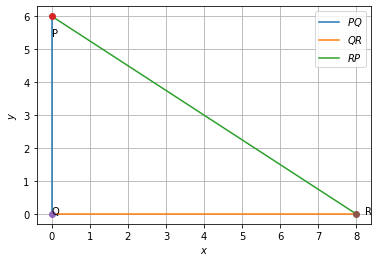
\includegraphics[width=\columnwidth]{solutions/24/Figure1.png}
\caption{Right Angle $\triangle PQR$}
\label{constr/24/fig:right_angle_triangle}	
\end{figure}
